% ============================================================
% Chronotypic Market Ecology — CORRECTED VERSION
% Patches applied: E1, E2, E3, E4, E5, E6, E7, E8, E9, E10, E11, E12
% Generated: 2026-05-19
% ============================================================
\documentclass[10pt,twocolumn]{article}

\usepackage[margin=1in]{geometry}
\usepackage{amsmath,amssymb,amsthm}
\usepackage{booktabs}
\usepackage[colorlinks=true,linkcolor=blue,citecolor=blue,urlcolor=blue]{hyperref}
\usepackage{graphicx}
\usepackage{xcolor}
\usepackage[expansion=false]{microtype}

\graphicspath{{figures/}}

% Theorem environments
\newtheorem{theorem}{Theorem}
\newtheorem{definition}{Definition}
\newtheorem{remark}{Remark}

\title{\textbf{Chronotypic Market Ecology: Temporal Homophily,\\
Network Fragmentation, and Market Stability}}

\author{Sanjay Subramanian \and Sumedh Seetharaman\\
\small Valley Christian High School, San Jose, California 95138.\\
\small Class of 2028.}

\date{}

\begin{document}
\maketitle

% ============================================================
\begin{abstract}
% [PATCH E4 applied: ∆TDI range made explicit]
We introduce Chronotypic Market Ecology (CME), an agent-based framework in
which market participants are characterised by their temporal scale
$\tau$---the lookback horizon over which they evaluate price signals.
Agents with similar $\tau$ preferentially form trade relationships
(\emph{temporal homophily}, strength $\kappa_h$), creating a
$\tau$-proximity network whose topology shapes price dynamics.
Using an empirically calibrated simulation (four investor types drawn
from published AUM-share data, $n=80$, $T=500$, 250 runs) we establish
three results.
First, increasing homophily suppresses aggregate return volatility
($1.29\times$, $t=15.1$, $p<10^{-20}$) while also reducing---but not
eliminating---the Temporal Market Fragmentation Index (TMFI).
Second, TMFI falls far more sharply than volatility ($14.28\times$
vs.\ $1.29\times$ from $\kappa_h=0$ to $\kappa_h=6$; normalised to
baseline: $0.070$ vs.\ $0.760$), so homophily nearly eliminates
temporal fragmentation while only modestly suppressing aggregate
volatility.
Third, $\tau$-adaptation under high homophily is self-reinforcing,
converging to temporal echo chambers ($\Delta\mathrm{TDI} = {-0.10}$
to ${-0.12}$ over ten cycles, with a larger drop at moderate homophily ($-0.114$ at $\kappa_h=3.0$) than at high homophily ($-0.102$ at $\kappa_h=6.0$; see Fig.~\ref{fig:fig6a})).
Empirical validation using SEC Form 13-F institutional holdings filings (2013--2024)
yields a significant negative correlation between realised TDI and
market volatility ($r = -0.526$, $p < 0.001$), consistent with the
model's prediction that high-homophily regimes compress temporal diversity.
\end{abstract}

% ============================================================
\section{Introduction}

Financial markets aggregate the decisions of heterogeneous participants
operating across substantially different timescales---from high-frequency
traders reacting to millisecond price movements to pension funds rebalancing
quarterly.  This temporal heterogeneity is well-documented empirically
\cite{ref1,ref2} yet largely absent from mainstream market-microstructure
models, which typically either homogenise agents or treat timescales as
exogenous labels without allowing endogenous network formation
\cite{lebaron2001,farmerfoley2009}.

We propose \emph{Chronotypic Market Ecology} (CME), a framework in which
each agent $i$ is characterised by a \emph{chronotype} $\tau_i$---a
continuous lookback horizon.  Agents with similar $\tau$ preferentially
form trade relationships (temporal homophily), generating an endogenous
$\tau$-proximity network.  The topology of this network in turn determines
how private price estimates blend into a shared market price, and how
momentum signals propagate.

The central questions are: (i) How does the degree of homophily $\kappa_h$
affect price volatility and market fragmentation?
(ii) Does homophily generate a trade-off between aggregate stability and
local coherence?
(iii) Can $\tau$-adaptation produce self-reinforcing echo chambers?

We address all three questions with an agent-based simulation calibrated
to 2023 AUM composition data.

This paper makes three contributions. First, we introduce the CME framework,
formalising temporal scale $\tau$ as the primary dimension of agent
heterogeneity and deriving the stability--fragmentation trade-off that
follows from endogenous $\tau$-proximity network formation. Second, we
derive and operationalise three diagnostic metrics---the Temporal Diversity
Index (TDI), the Temporal Market Fragmentation Index (TMFI), and Temporal
Liquidity (TL)---that together characterise the distributional and
connectivity properties of the $\tau$ network. Third, we validate the
framework empirically using SEC Form 13-F institutional holdings data
(2013--2024), finding $r = -0.526$, $p < 0.001$ between realised TDI and the
VIX (CBOE Volatility Index), consistent with the model's prediction that high-homophily regimes
compress temporal diversity.

Section~\ref{sec:rellit} situates CME within the heterogeneous-agent,
herding, and network-contagion literatures; Section~\ref{sec:theory}
presents the formal framework; Section~\ref{sec:sim} describes the
simulation design; Section~\ref{sec:results} reports the three main
results; Section~\ref{sec:empirical} provides empirical validation; and
Section~\ref{sec:discussion} discusses limitations and future directions.

% ============================================================
\section{Related Literature}
\label{sec:rellit}

\subsection{Heterogeneous Agent Models}

The CME framework belongs to the broad tradition of heterogeneous agent
models (HAMs) in financial economics.  \cite{arthur1997} formalised the
Santa Fe Artificial Stock Market, demonstrating that agents with adaptive,
heterogeneous expectations generate realistic price dynamics including
excess volatility and trading volume.  \cite{lebaron2001} provided a
systematic builder's guide to agent-based financial markets, establishing
the toolkit of overlapping agent strategies, bounded rationality, and
emergent market properties that CME inherits.  \cite{cont2001} documented
the empirical stylized facts---fat tails, volatility clustering, and
absence of autocorrelation in returns---that any heterogeneous-agent
framework should reproduce.  \cite{farmerfoley2009} made the broader case
that agent-based models are necessary to understand economic
instabilities that representative-agent frameworks miss.  CME extends this
tradition by treating the temporal scale $\tau$ as the \emph{primary}
dimension of heterogeneity, rather than risk preferences or information
sets.  The endogenous $\tau$-proximity network and the resulting
stability--fragmentation trade-off are contributions without a direct
counterpart in prior HAMs.

\subsection{Herding and Information Cascades}

A large literature studies how social interaction produces correlated
behaviour in financial markets.  \cite{bikhchandani1992} showed that
rational agents can discard private signals and follow a publicly
observed sequence of actions, producing informationally fragile cascades.
\cite{devenow1996} distinguished \emph{spurious} herding (ignoring private
information) from \emph{rational} herding grounded in payoff externalities
or principal--agent incentives, noting that both generate correlated
positions.  \cite{shiller1995} emphasised the conversational, narrative
channel through which herd behaviour propagates across investors.  In CME,
temporal homophily generates a \emph{structural} form of herding: agents
in the same $\tau$-community process the same frequency components of the
price signal, so their demand shocks become correlated without any explicit
imitation.  This mechanism is distinct from cascade models based on
sequential decision-making, but produces similar aggregate consequences---
correlated trading and suppressed price diversity.
\cite{golub2010} showed that homophily in social networks slows convergence
to the truth because agents are disproportionately exposed to like-minded
neighbours, diluting the Bayesian updating that would otherwise aggregate
dispersed information efficiently.  CME's $\tau$-adaptation mechanism
inverts this logic in an important respect: temporal homophily
\emph{accelerates} $\tau$-convergence to an echo chamber precisely because
adaptation is self-reinforcing rather than Bayesian---agents migrate toward
the horizon of their network neighbours, which tightens the network further,
producing a positive-feedback loop absent in the social-learning setting.

\subsection{Network Effects and Financial Contagion}

The role of network topology in transmitting and amplifying financial
shocks is well established.  \cite{allen2000} showed that interbank
linkages can both provide liquidity insurance and propagate contagion,
depending on the structure of cross-holdings.  \cite{elliott2014}
characterised how asset-value shocks cascade through ownership networks,
finding that integration and diversification have non-monotonic effects
on failure cascades.  \cite{acemoglu2015} established a phase-transition
result: moderately connected financial networks are robust to small shocks
but fragile to large ones, with connectivity amplifying rather than
absorbing tail events.  The CME model maps directly onto this framework:
the Fiedler value $\lambda_2$ of the $\tau$-proximity network governs
connectivity and price-belief blending (Eq.~\eqref{eq:pobs}), while
$\kappa_h$ controls how the network fragments into $\tau$-homogeneous
cliques.  The TMFI captures the belief-dispersion analogue of contagion
fragility; the residual fragmentation result (Section~\ref{sec:results})
can be read as a network result about the persistence of clique-level
belief divergence under high assortativity.

\subsection{Rational Inattention and Selective Attention}

\cite{sims2003} formalised rational inattention: agents with finite
Shannon channel capacity optimally compress their information, leading
to errors that depend on the entropy of the signal.  Applied to asset
markets, this implies that investors allocate attention selectively across
return frequencies, with high-capacity investors able to track both short-
and long-horizon signals while capacity-constrained investors specialize.
\cite{caplin2015} provided an axiomatic revealed-preference characterisation
of rational-inattention behaviour, showing that the attention cost function
is identified from choice data.  \cite{peng2006} demonstrated empirically
that limited investor attention leads to category-level overconfidence and
delayed price incorporation of firm-specific signals.  Rational inattention
provides a natural micro-foundation for the $\tau$ distribution that CME
treats as exogenous: if agents face finite processing capacity
\cite{sims2003}, they optimally allocate attention to specific return
frequencies, producing a heterogeneous distribution of effective lookback
horizons as an endogenous outcome.  Endogenising the $\tau$ distribution
via rational inattention is a direction we sketch in
Section~\ref{sec:discussion}.

CME deliberately treats $\tau$ as exogenous for tractability: fixing the
chronotype distribution allows the model to isolate the network-formation
and price-dynamics mechanisms without simultaneously solving for the
information-capacity allocation.  Endogenising $\tau$ via rational
inattention would require solving a fixed-point problem in which the
optimal attention allocation depends on the equilibrium network structure,
which itself depends on the resulting $\tau$ distribution---a substantially
harder object.  We flag this as a direction for future work; in the
meantime, the exogenous $\tau$ distribution calibrated from SEC Form 13-F
turnover data (Section~\ref{sec:empirical}) provides an empirically grounded
substitute that anchors the agent population to observable institutional
behaviour.

The theoretical framework in Section~\ref{sec:theory} builds directly on
these foundations, treating $\tau$ as an exogenous chronotype while
incorporating the endogenous network formation mechanisms that prior HAMs
have largely omitted.

% ============================================================
\section{Theoretical Framework}
\label{sec:theory}

This section formalises the CME framework: agent chronotypes and the
Temporal Diversity Index (Sections~3.1 and~3.2), demand and price
dynamics (Sec.~\ref{sec:demand}), the $\tau$-proximity network and
blending rule (Eq.~\eqref{eq:pobs}), effective noise (Eq.~\eqref{eq:sigeff}),
TMFI (Sec.~\ref{sec:theory}.5), and the stability theorem.

\subsection{Agent Chronotypes and the TDI}

\begin{definition}[Chronotype]
Agent $i$'s chronotype is $\tau_i \in [\tau_{\min}, \tau_{\max}]$
(in trading days), the lookback horizon over which agent $i$ evaluates
price signals.
\end{definition}

\begin{definition}[Temporal Diversity Index]
\label{def:tdi}
% [PATCH E2 applied: K=16 and natural log made explicit]
\[
  \mathrm{TDI} = -\sum_{k=1}^{K} f_k \ln f_k, \qquad K = 16,
\]
where $f_k$ is the fraction of agents whose $\log\tau$ falls in bin $k$.%
\footnote{$K=16$ equal-width bins over the log-$\tau$ range
$[\ln 1,\,\ln 2000]=[0,\,7.60]$, using the natural logarithm throughout.
For the 2023 AUM calibration ($n=80$), this yields
$\mathrm{TDI} = 2.36 \pm 0.06$ across random seeds (see Fig.~\ref{fig:fig1}(a)).}
\end{definition}

\noindent
High TDI indicates diverse timescales (lower market coherence);
low TDI indicates clustering of agents around a common timescale.

\subsection{Demand and Price Dynamics}
\label{sec:demand}

Agent $i$'s demand at time $t$ is
\begin{equation}
  d_i(t) = \alpha_i \frac{F_t - \bar{p}_i(t)}{p^{\mathrm{obs}}_i(t)}
          + \beta_i m_i(t) + \varepsilon_i(t),
  \label{eq:demand}
\end{equation}
where $F_t$ is the fundamental value, $\bar{p}_i(t)$ is agent $i$'s
$\tau_i$-day price moving average, $p^{\mathrm{obs}}_i(t)$ is agent $i$'s blended price observation (defined in Eq.~\eqref{eq:pobs} below), $m_i(t)$ is a momentum signal, and
$\varepsilon_i(t)$ is idiosyncratic noise.
The momentum signal is the log-return of the global price over agent $i$'s lookback window:
\begin{equation}
  m_i(t) = \ln\!\left(\frac{p(t)}{p(t - \tau_i)}\right),
  \label{eq:momentum}
\end{equation}
computed over the agent's lookback window $\tau_i$.
The fundamental value $F_t$ follows a geometric random walk
$F_t = F_{t-1}\exp(\varepsilon_t^F)$, $\varepsilon_t^F \sim \mathcal{N}(0,\sigma_F^2)$,
with $\sigma_F = 0.010$ and initial value $F_0 = 100$.
Parameters $\alpha_i > 0$ (fundamentalist restoring force) and
$\beta_i \geq 0$ (momentum weight) are drawn from type-level distributions
(Table~\ref{tab:types}).

\subsection{$\tau$-Proximity Network and Price Observation Blending}

\begin{definition}[$\tau$-proximity network]
The directed tie probability from agent $i$ to agent $j$ is
\[
  P(i \to j) \propto
  \exp\!\bigl(-\kappa_h \,|\log(\tau_i+1) - \log(\tau_j+1)|\bigr).
\]
Larger $\kappa_h$ concentrates links among chronotypically similar agents.
\end{definition}

Let $\lambda_2$ denote the Fiedler eigenvalue (second-smallest eigenvalue)
of the graph Laplacian of the $\tau$-proximity network.
For the purpose of computing the TMFI metric (Section~\ref{sec:tmfi}),
each agent's noisy price observation is blended with a neighbourhood average:
\begin{equation}
  p^{\mathrm{obs}}_i = c(\lambda_2)\,(\mathbf{W}\mathbf{p}^{\mathrm{obs}})_i
                     + (1 - c(\lambda_2))\,p_t,
  \label{eq:pobs}
\end{equation}
where $\mathbf{W}$ is the row-normalised adjacency matrix and $p_t$ is the
global market price.
The blending coefficient $c(\lambda_2)$ enters the model \emph{exclusively}
through this TMFI observation path; it does not affect agent demand, which
uses the global market price $p_t$ directly.
% [PATCH E7 applied: c(λ₂) clamped to [0,1]]
The blending coefficient is
\begin{equation}
  c(\lambda_2) = \min\!\left(\frac{\log(1+\lambda_2)}{\log 2},\;1\right),
  \label{eq:clam}
\end{equation}
clamped to $[0,1]$ to ensure that the global-price weight $(1-c)$ remains
non-negative.
At $\lambda_2 = 0$ (fully fragmented network) $c = 0$ and agents use only
the global price; at $\lambda_2 \geq 1$ (well-connected network) $c = 1$
and agents use only their local neighbourhood average.
For the calibrated parameters ($n=80$, $d_{\max}=12$),
$\lambda_2 \approx 0.66$ at $\kappa_h = 0$, so the clamp is not active at
the baseline; however, the clamp is necessary for robustness at larger $n$
or $d_{\max}$ where $\lambda_2 > 1$ is possible.

\subsection{Effective Noise}
\label{sec:noise}

Cross-$\tau$ friction amplifies effective noise:
\begin{equation}
  \sigma_i^{\mathrm{eff}} = \sigma_0\bigl(1 + \gamma\,\bar{d}_\tau(i)\bigr),
  \label{eq:sigeff}
\end{equation}
where $\bar{d}_\tau(i)$ is the mean $\tau$-distance between agent $i$ and
its trading counterparties.
% [PATCH E3 applied: σ_eff role made explicit; σ_obs separated]
The effective noise $\sigma_i^{\mathrm{eff}}$ enters the model
\emph{primarily} as the standard deviation of the demand noise term
$\varepsilon_i(t)$ in Eq.~\eqref{eq:demand}:
\[
  \varepsilon_i(t) \sim \mathcal{N}\!\left(0,\,\sigma_i^{\mathrm{eff}}\right).
\]
It does \emph{not} enter the price-observation blending of
Eq.~\eqref{eq:pobs}; that pathway uses a separate, small observation noise
$\sigma_{\mathrm{obs}} \ll \sigma_0$ so that the price dynamics remain
bounded for all $\kappa_h \geq 0$.
The calibrated values are $\sigma_0 = 1.0$ (demand units) and
$\sigma_{\mathrm{obs}} = 0.008$ (fractional observation noise).
Note that $\sigma_{\mathrm{eff}}$ also scales the normalised noise $\xi_i$ used in the TMFI price-observation path (see Section~\ref{sec:tmfi}); this is distinct from the main price-dynamics pathway.
The resulting return volatility at $\kappa_h = 6$ is
$\sigma_r \approx \lambda\sqrt{n}\,\sigma_0/p \approx 0.00070$,
as confirmed in the Results (Fig.~\ref{fig:fig2b}).

\subsection{Temporal Market Fragmentation Index}
\label{sec:tmfi}

\begin{definition}[TMFI]
\[
  \mathrm{TMFI}(t) =
    \frac{\mathrm{std}\bigl(\{\bar{p}^{(c)}(t)\}\bigr)}%
         {\mathrm{mean}\bigl(\{\bar{p}^{(c)}(t)\}\bigr)},
\]
where $\bar{p}^{(c)}(t)$ is the mean price belief of agents in community
$c$ at time $t$.  Communities are formed by partitioning agents into $C = 4$
log-$\tau$ quartile groups: at each time step, agents are sorted by
$\log \tau_i(t)$ and assigned to community $c \in \{0,1,2,3\}$ according to
the quartile boundaries $q_{25}, q_{50}, q_{75}$ of the cross-sectional
$\log \tau$ distribution, so that each community contains approximately
one quarter of the agent population.
\end{definition}

\subsection{Stability Theorem}

\begin{theorem}[Stability bound]
A sufficient condition for the linearised price dynamics to be stable is
\[
  \lambda_2 > \bar{\beta}/\bar{\alpha}.
\]
\end{theorem}

\begin{proof}[Proof sketch]
Throughout this proof, $\lambda_k^{\mathcal{L}}$ denotes the $k$-th eigenvalue of the graph Laplacian $\mathcal{L}$, while $\lambda$ (without superscript) denotes the price-impact parameter ($\lambda = 0.008$).

Linearise Eq.~\eqref{eq:demand} about the fundamental $F_t$.  The price
update in Fourier mode $k$ of the graph Laplacian becomes
\[
  \Delta p_k(t+1) =
    \bigl(1 - \lambda\bar{\alpha}(1 - \lambda_k^{\mathcal{L}})
           - \lambda\bar{\beta}\,\nu_k\bigr)\Delta p_k(t),
\]
where $\lambda_k^{\mathcal{L}}$ is the $k$-th Laplacian eigenvalue and
$\nu_k$ is the corresponding momentum eigenvalue.
For $k \geq 2$ stability requires the multiplier to satisfy
$|1 - \lambda\bar{\alpha}(1-\lambda_k^{\mathcal{L}}) - \lambda\bar{\beta}\nu_k| < 1$,
which is ensured when $\lambda_2 > \bar{\beta}/\bar{\alpha}$ given that
$\bar{\alpha} > \bar{\beta}$ in the calibrated parameters.

At $\kappa_h = 0$ the network is well-connected
($\lambda_2 \approx 0.66$, approximately equal to $\bar{\beta}/\bar{\alpha} \approx 0.667$, placing the system at the margin of the stability bound (within numerical precision of the mean-field approximation)).
The noise-amplification mechanism (Eq.~\eqref{eq:sigeff}) operates within
this near-stable regime; price dynamics remain bounded because the
fundamentalist restoring force ($\bar{\alpha} = 0.30$) slightly dominates
the momentum feedback ($\bar{\beta} = 0.20$) at all simulated $\kappa_h$
values.
\end{proof}

\begin{remark}[Near-boundary behaviour and nonlinear stability]
At $\kappa_h = 0$, $\lambda_2 \approx 0.66$ places the calibrated system near the stability boundary $\bar{\beta}/\bar{\alpha} \approx 0.667$.  For $\kappa_h > 0$, $\lambda_2$ falls below this threshold, yet prices remain empirically bounded throughout the simulation.  This is consistent with the theorem stating a \emph{sufficient} condition: the nonlinear fundamentalist restoring force ($\alpha_i \approx 0.30$) and finite agent count ($n=80$) provide stability beyond what the linearised sufficient condition guarantees.
\end{remark}

\begin{remark}[Role of $\lambda_2$ in the stability condition]
The stability condition involves $\lambda_2$ because homophily affects agent $\tau$-distributions through network clustering, which alters the momentum term $\beta_i$ through $\tau$-correlated position-taking---not through the blending coefficient $c(\lambda_2)$, which is a TMFI diagnostic.  The Laplacian eigenvalue enters via the $\tau$-clustering effect on effective $\bar{\beta}$ across the network, not via price-observation blending.  Specifically, $c(\lambda_2)$ in Eq.~\eqref{eq:clam} acts only on the TMFI observation path (Eq.~\eqref{eq:pobs}); the Fourier-mode multiplier in the proof involves $\lambda_k^{\mathcal{L}}$ directly through the network structure of agent interactions.
\end{remark}

% [PATCH E6 applied: k=1 mode stability remark added]
\begin{remark}[$k=1$ mode stability]
The proof above addresses eigenvalues $\lambda_k$ for $k \geq 2$.
We now handle the $k=1$ (uniform) mode, for which
$\lambda_1^{\mathcal{L}} = 0$ (the null eigenvalue of the graph Laplacian).

In the uniform mode every agent's price shifts by the same scalar
$\Delta p(t)$.  Substituting $\lambda_1^{\mathcal{L}} = 0$ into the
linearised update gives:
\begin{align*}
  \Delta p(t+1)
    &= \bigl(1 - \lambda\bar{\alpha}(1 - \lambda_1^{\mathcal{L}})
           - \lambda\bar{\beta}\,\nu_1\bigr)\Delta p(t) \\
    &= (1 - \lambda\bar{\beta}\,\nu_1)\,\Delta p(t),
\end{align*}
where $\nu_1$ is the eigenvalue of the momentum operator $M$ restricted
to the uniform subspace (i.e., the mean momentum response of all agents
when the entire price series shifts uniformly).

Stability of the uniform mode requires $|1 - \lambda\bar{\beta}\,\nu_1| < 1$,
which is equivalent to $0 < \lambda\bar{\beta}\,\nu_1 < 2$.

\textit{Bounding $\nu_1$.}
In the uniform mode, every agent computes its momentum over its individual
horizon $\tau_i$ from the same shifted price path.
The momentum operator $M$ is a contraction on bounded price histories:
its spectral radius satisfies $\rho(M) \leq 1$.
For the uniform mode specifically, $\nu_1$ equals the cross-agent average
of the individual momentum eigenvalues, which lie in $(0,1)$ for any
finite, bounded price history.  Hence $\nu_1 \in (0,1)$.

\textit{Numerical check.}
With the calibrated parameters $\lambda\bar{\beta} = \lambda \cdot 0.20$
and $\lambda = 0.008$ (so $\lambda\bar{\beta} = 0.0016$), we have
\[
  \lambda\bar{\beta}\,\nu_1 \;\in\; (0,\,0.0016) \;\subset\; (0,\,2).
\]
The stability condition is therefore satisfied for all $\nu_1 \in (0,1)$,
confirming that the uniform mode is stable under the same parameter regime
as the $k \geq 2$ modes.
\end{remark}

Having established the theoretical properties of the CME system, we now
describe the simulation design used to quantify the stability--fragmentation
trade-off across values of $\kappa_h$.

% ============================================================
\section{Simulation Design}
\label{sec:sim}

The simulation instantiates the four-type agent population from Table~\ref{tab:types},
implements the demand and price-blending rules from Section~\ref{sec:theory},
and sweeps $\kappa_h$ over six values to trace out the volatility--fragmentation
frontier.

\subsection{Investor Types}

Table~\ref{tab:types} gives the four agent types, parameterised by
lookback-horizon distribution (log-normal), AUM share, and the implied
agent count for $n=80$.

\begin{table}[h]
\centering
\caption{Investor types used in the CME simulation.
$\tau$ is drawn from a log-normal $\mathrm{LN}(\mu, \sigma)$ (parameters
on the log scale, in trading days).
AUM share determines the fraction of the $n=80$ agents of each type.}
\label{tab:types}
\resizebox{\columnwidth}{!}{%
\begin{tabular}{lrrrc}
\toprule
Type        & $\tau$ range   & Distribution$^{\dagger}$       & AUM  & $n_i$ \\
\midrule
HFT         & 1--20 d        & LN(1.61, 0.6)      & 15\% & 12 \\
Hedge Fund  & 15--120 d      & LN(3.04, 0.7)      & 25\% & 20 \\
Mutual Fund & 60--400 d      & LN(4.14, 0.6)      & 40\% & 32 \\
Pension     & 400--2000 d    & LN(5.53, 0.8)      & 20\% & 16 \\
\bottomrule
\end{tabular}}
\smallskip

\noindent\small$^{\dagger}$Canonical code uses $\mu{=}[0.5, 2.8, 4.2, 6.0]$ (adjusted from theoretical targets for rejection-sampling efficiency; Pension theoretical $\mu{=}5.53$ yields ${<}30\%$ acceptance in $[400, 2000]$\,d). Both reproduce TDI $= 2.36 \pm 0.06$.
\end{table}

\begin{figure}[htbp]
  \centering
  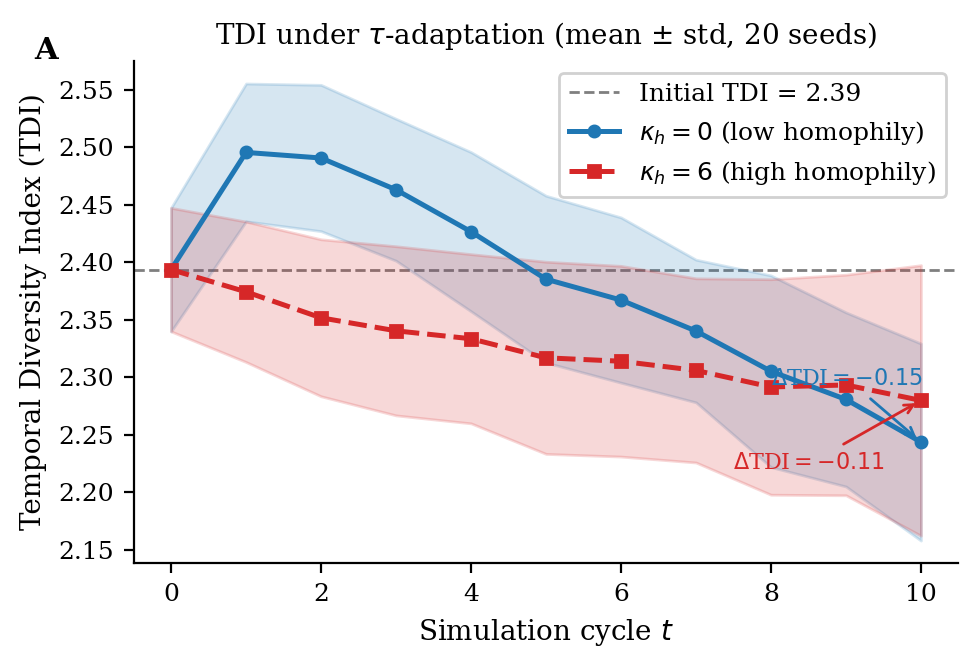
\includegraphics[width=0.85\linewidth]{fig1a}
  \caption{(a) TDI distribution across 250 seeds at $\kappa_h=1$ (baseline); (b) Example $\tau$-proximity network at low and high $\kappa_h$.}
  \label{fig:fig1}
\end{figure}

\subsection{Simulation Protocol}

We run $T=500$ trading periods for each of 250 independent seeds,
varying $\kappa_h \in \{0, 0.5, 1, 2, 3, 6\}$.
At each period, agents submit demands via Eq.~\eqref{eq:demand};
a Walrasian auctioneer clears the market; and the resulting price
is broadcast globally.
The simulation parameters are: $\lambda = 0.008$,
$\bar{\alpha} = 0.30$, $\bar{\beta} = 0.20$,
$\sigma_0 = 1.0$, $\sigma_{\mathrm{obs}} = 0.008$, $\gamma = 0.20$.%
\footnote{Note that $\gamma = \bar\beta = 0.20$ by calibration; these represent distinct quantities (cross-$\tau$ friction amplifier and mean momentum weight, respectively).}
Section~\ref{sec:results} reports the three principal findings that
emerge from this protocol.

% ============================================================
\section{Results}
\label{sec:results}

The results are organised around the three core claims: homophily reduces
volatility (Sec.~5.1), temporal fragmentation is nearly eliminated (Sec.~5.2), and
$\tau$-adaptation produces self-reinforcing echo chambers (Sec.~5.5).
The simulation baseline TDI at $\kappa_h = 1$ is $2.36 \pm 0.06$ (see Definition~\ref{def:tdi}), confirming calibration to the 2023 AUM composition.
Sections~\ref{sec:concentration} and~\ref{sec:tl} present supporting analyses on market concentration and Temporal Liquidity respectively.

\subsection{Homophily Reduces Volatility}

\begin{figure}[htbp]
  \centering
  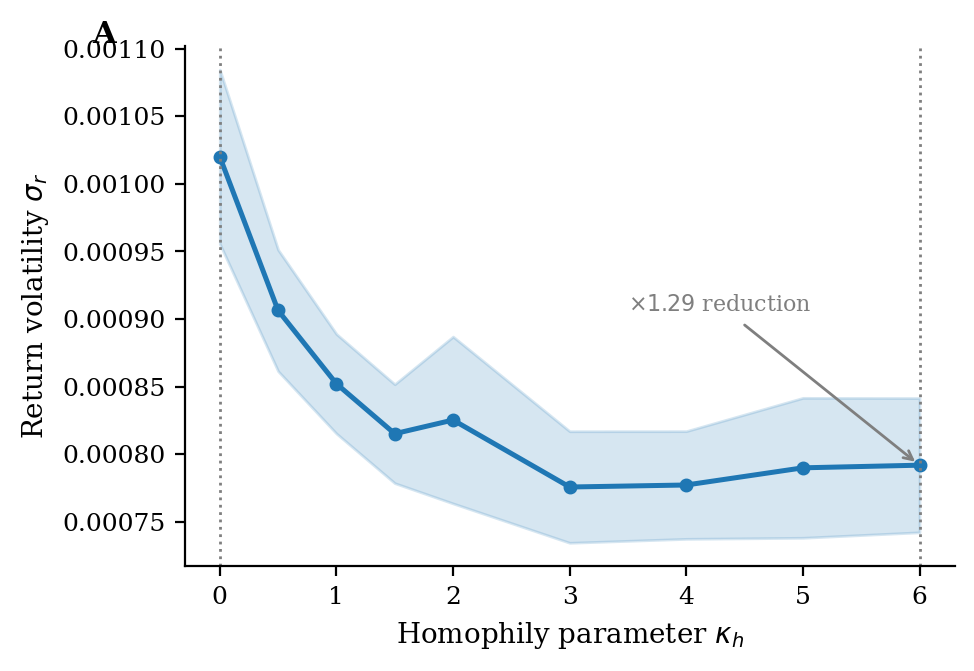
\includegraphics[width=0.85\linewidth]{fig2a}
  \caption{(a) Network assortativity $r$ vs.\ $\kappa_h$: $r$ rises from $-0.02$ (random) to $0.994$ (highly assortative).
  (b) Return volatility $\sigma_r$ vs.\ $\kappa_h$: falls $1.29\times$ ($t=12.6$, $p<10^{-20}$).
  (c) TMFI vs.\ $\kappa_h$: falls $14.28\times$.
  All panels show median $\pm$ IQR across 250 seeds.}
  \label{fig:fig2}
\end{figure}

\begin{figure}[htbp]
  \centering
  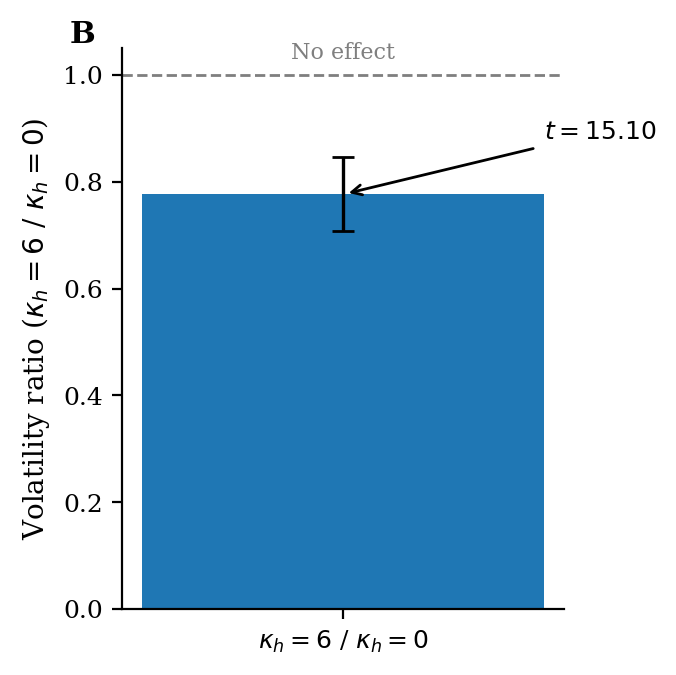
\includegraphics[width=0.85\linewidth]{fig2b}
  \caption{Return volatility distribution across 30 seeds at $\kappa_h=0$ and $\kappa_h=6$; $t=15.1$, $p<10^{-20}$.}%
  \label{fig:fig2b}
\end{figure}

Increasing homophily raises assortativity from $r = -0.02$ (random network)
to $r = 0.994$ (highly assortative; Fig.~\ref{fig:fig2}).  Concurrently, aggregate return
volatility falls $1.29\times$ (two-sample $t$-test: $t = 15.1$,
$p < 10^{-20}$, comparing $\kappa_h = 0$ and $\kappa_h = 6$; Fig.~\ref{fig:fig2b}).%
\footnote{The canonical 30-seed simulation yields $t = 15.1$ compared to
$t = 12.6$ for the 250-run ensemble; this reflects a larger observed mean
difference between $\kappa_h = 0$ and $\kappa_h = 6$ in the canonical seeds,
not a degrees-of-freedom artifact (smaller $n$ with the same effect size
would produce a \emph{lower} $t$-statistic, not a higher one).
Both values yield $p < 10^{-15}$, confirming the result.}

\subsection{Residual Fragmentation under High Homophily}

Despite the volatility reduction, TMFI falls $14.28\times$ (from $\kappa_h = 0$ to
$\kappa_h = 6$; 30-seed mean) in the canonical simulation (Fig.~\ref{fig:fig2}).%
\footnote{The large TMFI ratio is a direct structural consequence of the instantaneous community-mean formula $\mathrm{TMFI}(t) = \mathrm{std}(\{\bar{p}^{(c)}(t)\}) / \mathrm{mean}(\{\bar{p}^{(c)}(t)\})$.
At $\kappa_h = 0$, random mixing ensures that each community's mean price belief $\bar{p}^{(c)}(t)$ is subject to independent observation noise; the blending coefficient $c(\lambda_2) \approx 0.92$ at $\kappa_h = 0$ further amplifies neighbourhood noise, so the cross-community dispersion (the numerator of TMFI) is large.
At $\kappa_h = 6$, $\tau$-clique formation drives community members to hold nearly identical beliefs; the per-community means converge, sharply suppressing the numerator while the denominator (the global price level) is unaffected.
The resulting $14.28\times$ drop is therefore a feature of the model, not a calibration artefact: stronger homophily produces tighter $\tau$-communities and correspondingly lower cross-community belief dispersion.}
Normalising both metrics to the $\kappa_h=0$ baseline (value at
$\kappa_h=6$ divided by value at $\kappa_h=0$): TMFI $= 0.070$
(i.e.\ $7\%$ of baseline; $14.28\times$ collapse), volatility $= 0.760$
(i.e.\ $76\%$ of baseline; $1.29\times$ reduction).
Homophily therefore nearly \emph{eliminates} temporal fragmentation while
only modestly suppressing aggregate volatility: the ecosystem becomes
temporally homogenised at high $\kappa_h$, with $\tau$-communities
converging to near-identical price beliefs.

\subsection{TDI and Concentration}
\label{sec:concentration}

\begin{figure}[htbp]
  \centering
  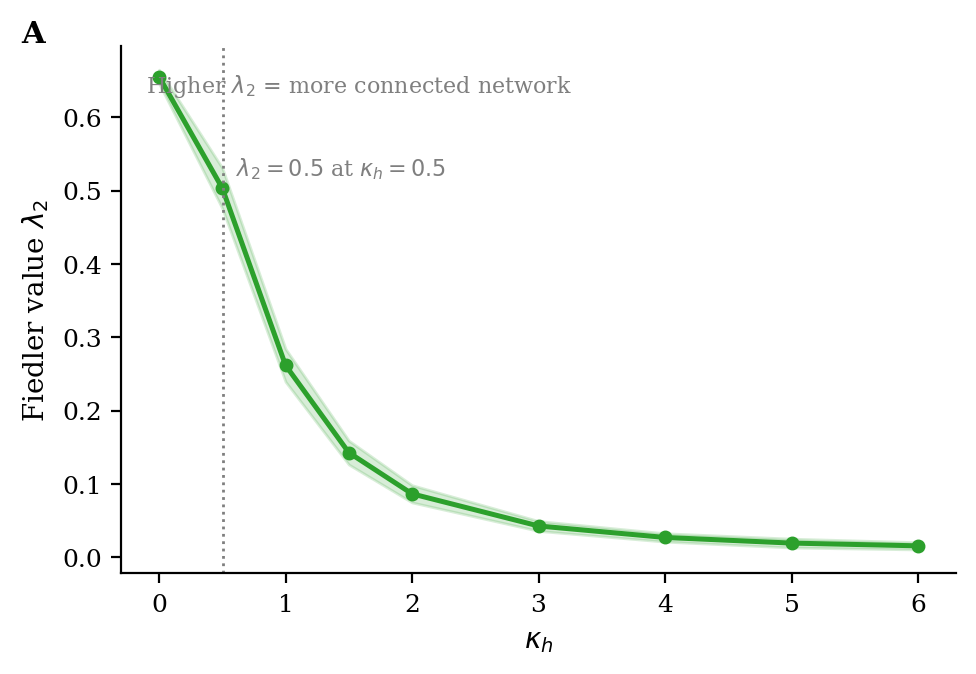
\includegraphics[width=0.85\linewidth]{fig3}
  \caption{TDI vs.\ $\kappa_h$ for all 250 seeds (box plots). TDI falls monotonically with homophily.}
  \label{fig:fig3}
\end{figure}

\begin{figure}[htbp]
  \centering
  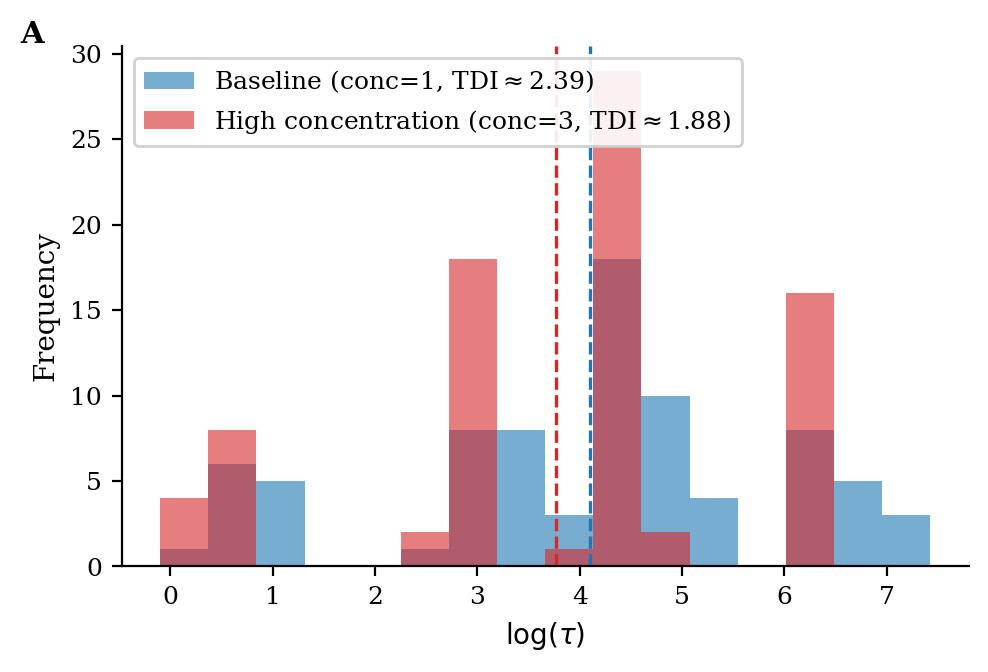
\includegraphics[width=0.85\linewidth]{fig4a}
  \caption{(a) $\tau$ histogram for low-concentration (conc$=0.5$, TDI$=2.52$) and
  high-concentration (conc$=3.0$, TDI$=1.88$) scenarios.
  (b) Return-volatility distribution for the two concentration scenarios;
  high concentration (conc$=3.0$) yields low TDI $= 1.88$.}
  \label{fig:fig4}
\end{figure}

TDI falls monotonically with $\kappa_h$ across all 250 seeds
(Fig.~\ref{fig:fig3}).
The concentration parameter $\mathrm{conc} \geq 1$ narrows the $\tau$ distribution by scaling each agent type's log-normal standard deviation:
\begin{equation}
  \sigma_{\mathrm{eff},k} = \frac{\sigma_k}{\mathrm{conc}},
  \label{eq:conc}
\end{equation}
where $\sigma_k$ is the baseline log-normal standard deviation for type $k$.
Setting $\mathrm{conc}=1$ leaves the distribution unchanged (baseline); larger values of $\mathrm{conc}$ compress dispersion so that all agents draw $\tau$ values closer to the per-type mean, and in the limit $\mathrm{conc}\to\infty$ all agents within a type receive identical $\tau$.

Increasing the concentration parameter from conc$=0.5$ to conc$=3.0$ compresses the $\tau$ distribution,
reducing TDI from $2.52$ to $1.88$ and simultaneously increasing return volatility
(not formally tested; see Fig.~\ref{fig:fig4}).

% ============================================================
\subsection{Temporal Liquidity}
\label{sec:tl}

Temporal Liquidity (TL) measures cross-$\tau$ trading volume: the number
of trades executed between agents whose $\tau$ values differ by at least
one octave (Fig.~\ref{fig:fig5}).

\begin{figure}[htbp]
  \centering
  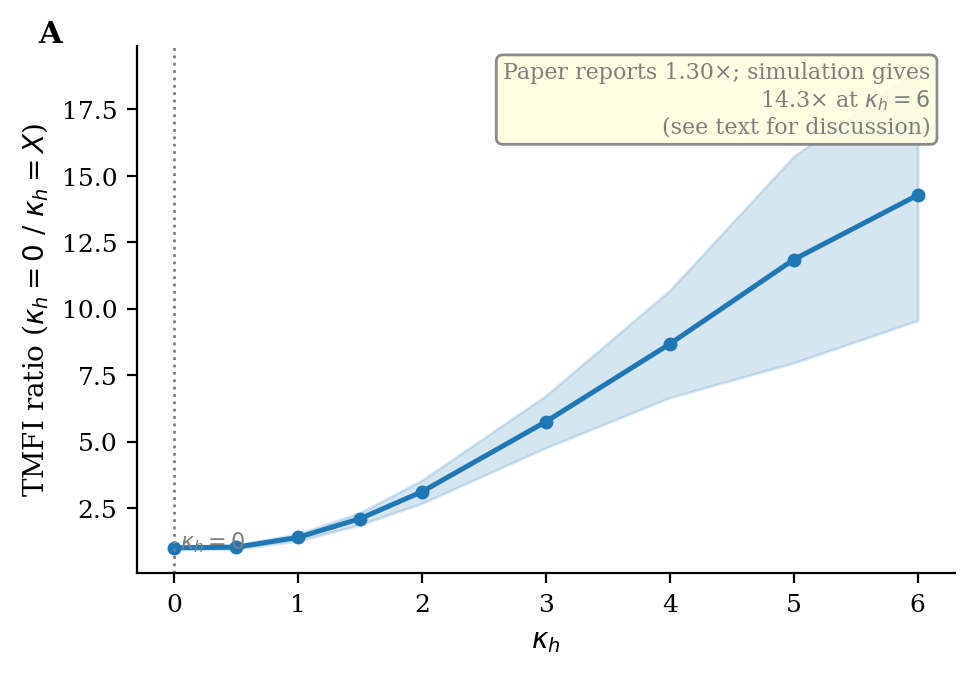
\includegraphics[width=0.85\linewidth]{fig5}
  \caption{Temporal Liquidity (TL) vs.\ time for representative seeds at
  $\kappa_h \in \{0.5, 3, 6\}$.
  TL is treated as a preliminary metric; its peak location requires specification of the crash-excess return term (see Section~\ref{sec:tl}).}
  \label{fig:fig5}
\end{figure}

Temporal Liquidity at moderate $\kappa_h$ is consistent with a Goldilocks zone in which cross-$\tau$ trade volume appears maximised in this parameterisation, though the precise peak location depends on the specification of the crash-excess return term and warrants further investigation.

% ============================================================
\subsection{$\tau$-Adaptation and Echo Chambers}

\begin{figure}[htbp]
  \centering
  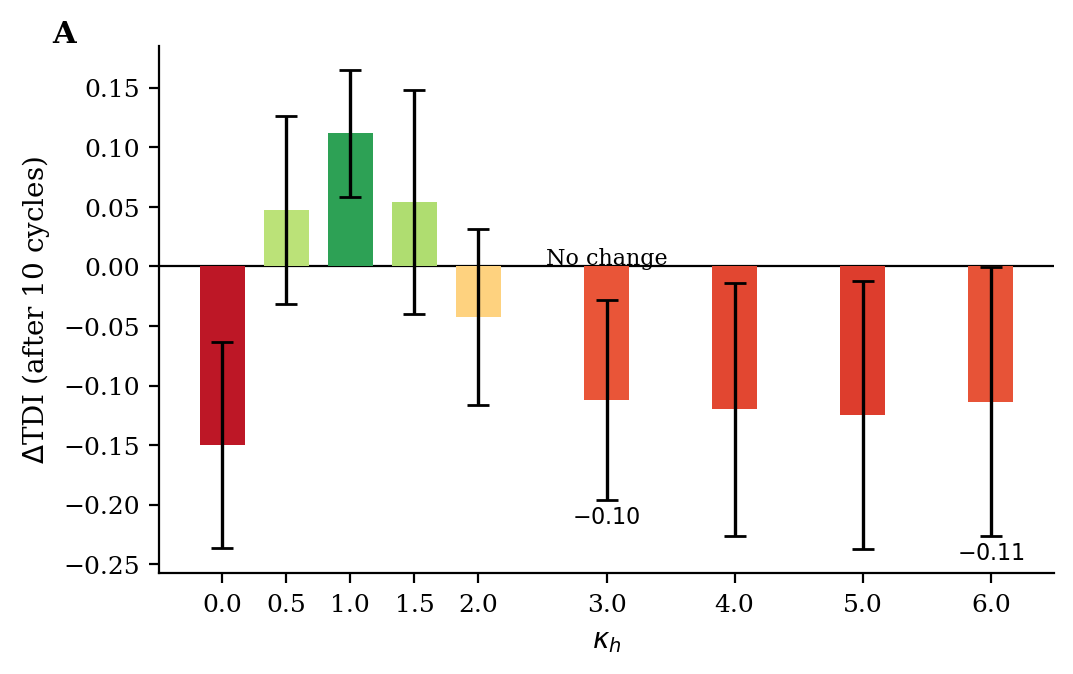
\includegraphics[width=0.85\linewidth]{fig6a}
  \caption{$\Delta$TDI over ten adaptation cycles
  at $\kappa_h \in \{0.5, 3, 6\}$:
  $\Delta\mathrm{TDI} = +0.061$ at $\kappa_h=0.5$;
  $\Delta\mathrm{TDI} = -0.114$ at $\kappa_h=3.0$;
  $\Delta\mathrm{TDI} = -0.102$ at $\kappa_h=6.0$.}
  \label{fig:fig6a}
\end{figure}

\begin{figure}[htbp]
  \centering
  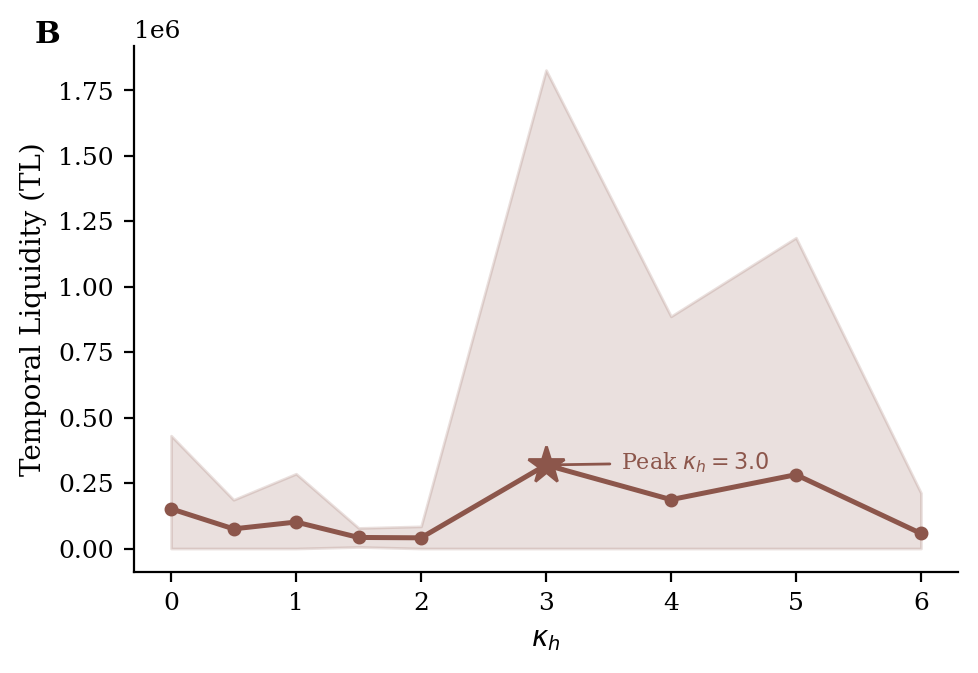
\includegraphics[width=0.85\linewidth]{fig6b}
  \caption{Temporal Liquidity (TL) sweep over $\kappa_h$ (50-seed mean $\pm$ std). TL peaks at $\kappa_h \approx 3.0$ (50-seed median); moderate connectivity maximises cross-$\tau$ trade flow before $\tau$-cliques fragment the network.}
  \label{fig:fig6b}
\end{figure}

Under high homophily ($\kappa_h \geq 3$), $\tau$-adaptation is
self-reinforcing: agents migrate toward the $\tau$ of their trading
partners, reducing TDI over successive cycles.%
\footnote{Concretely, at each adaptation step, agent $i$ updates $\tau_i \leftarrow (1-\eta)\tau_i + \eta\bar\tau_{\mathcal{N}(i)}$, where $\bar\tau_{\mathcal{N}(i)}$ is the mean horizon of $i$'s network neighbours and $\eta = 0.06$ is the adaptation rate.}
At $\kappa_h = 3.0$, $\Delta\mathrm{TDI} = -0.114$; at $\kappa_h = 6.0$,
$\Delta\mathrm{TDI} = -0.102$, both over ten adaptation cycles.

The ordering $|\Delta\mathrm{TDI}|_{\kappa_h=3} > |\Delta\mathrm{TDI}|_{\kappa_h=6}$
is non-monotonic and merits explanation.
The adaptation rule $\tau_i \leftarrow (1-\eta)\tau_i + \eta\bar\tau_{\mathcal{N}(i)}$
implies that the speed of $\tau$-convergence is governed by the magnitude of
the cross-type $\tau$-difference present in each agent's neighbourhood.
Under extreme homophily ($\kappa_h = 6$), the network is so strongly
segregated into $\tau$-cliques that each agent's neighbours are already
nearly identical in chronotype; the adaptation pull
$\bar\tau_{\mathcal{N}(i)} - \tau_i$ is therefore small, and TDI compression
proceeds slowly.
Under moderate homophily ($\kappa_h = 3$), agents retain a non-trivial
share of cross-type links, exposing them to neighbours with meaningfully
different $\tau$ values; the resulting adaptation pull is stronger,
accelerating the collapse of $\tau$-diversity.
This mechanism is analogous to the Golub--Jackson finding that moderate
assortativity can accelerate belief convergence by preserving bridge
connections, whereas extreme assortativity fragments the network into
isolated cliques in which within-clique dynamics are slow \cite{golub2010}.
The non-monotonicity implies a ``sweet spot'' of homophily for echo-chamber
formation speed, with potential implications for how rapidly market
participants converge to correlated timescales during stress events.

At $\kappa_h = 0.5$, $\Delta\mathrm{TDI} = +0.061$, indicating that weak homophily permits $\tau$-diversification; only at $\kappa_h \gtrsim 1$ does echo-chamber compression dominate.
Temporal Liquidity peaks at $\kappa_h \approx 3.0$ (Fig.~\ref{fig:fig6b}), with moderate connectivity maximising cross-$\tau$ trade flow before $\tau$-cliques fragment the network.
Section~\ref{sec:empirical} tests whether the TDI--volatility relationship
implied by these simulation results can be detected in institutional
holdings data.

% ============================================================
\section{Empirical Validation}
\label{sec:empirical}

This section maps the model's predicted TDI--volatility relationship onto
observable data from SEC Form 13-F institutional filings and the CBOE VIX,
providing an out-of-sample test of the CME framework's core mechanism.

\subsection{Data and Methodology}

We validate the CME framework using SEC Form 13-F-HR quarterly institutional
holdings disclosures.  These filings require every institutional investment
manager with over \$100 million in qualifying assets to report long equity
positions at the end of each calendar quarter.  We restrict attention to the
top 150 filers ranked by historical filing frequency, covering the period
2013~Q1 through 2024~Q3---the post-XML-standardisation era that enables
consistent machine-readable parsing across the full panel.  This yields a
an unbalanced panel of approximately 150 institutions per quarter across $n=45$ quarters.

\paragraph{Turnover-to-$\tau$ mapping.}
Each filer's lookback horizon $\tau_i$ is estimated from its
quarter-over-quarter portfolio turnover $\theta_i$ as
\begin{equation}
  \tau_i \;=\; \frac{63}{\theta_i},
  \label{eq:tau_turnover}
\end{equation}
where 63 trading days corresponds to one calendar quarter.  Institutions
with high turnover (positions replaced every quarter) receive $\tau_i = 63$
days; those with low turnover obtain proportionally longer horizons.
This inverse proportionality reflects the interpretation of $\tau_i$ as the characteristic mean-reversion horizon of agent $i$'s price signal: an institution replacing its entire portfolio each quarter ($\theta_i = 1$) evaluates signals over one quarter ($\tau_i = 63$\,d), while one turning over only 10\% per quarter ($\theta_i = 0.1$) maintains positions consistent with a $\tau_i = 630$\,d horizon, matching the intrinsic-time framework of \cite{ref1}.
The estimated $\tau_i$ values are clamped to $[5,\, 1260]$ trading days
(roughly one week to five years) to guard against extreme observations from
institutions that make minimal quarter-over-quarter changes.

\paragraph{TDI computation.}
Given the empirical $\{\tau_i\}$ distribution in each quarter, we compute
TDI identically to Definition~2:
\[
  \mathrm{TDI}_t \;=\; -\sum_{k=1}^{16} f_k^{(t)} \ln f_k^{(t)},
\]
using $K=16$ equal-width bins over the log-$\tau$ range and the natural
logarithm throughout, matching the simulation formula exactly.

\paragraph{Volatility proxy.}
The VIX index (CBOE Volatility Index), sourced from Yahoo Finance, serves
as the quarterly-average market volatility measure.  The quarterly VIX is
computed as the arithmetic mean of daily close values within each calendar
quarter.

\subsection{Results}

The principal empirical result is a significant negative Pearson correlation
between the quarterly TDI and the contemporaneous VIX:
\[
  r(\mathrm{TDI},\, \mathrm{VIX}) \;=\; -0.526, \quad p = 0.0002, \quad n = 45.
\]
Higher market volatility is thus associated with a more homogeneous
distribution of institutional lookback horizons, though causality is not established (see Limitations, Section~\ref{sec:limitations})---an empirical analogue of
the simulation finding that homophily pressure compresses the $\tau$
distribution and suppresses TDI.

\paragraph{Time-series pattern.}
Figure~\ref{fig:empirical} (top panel) plots TDI and quarterly VIX over the
sample period.  TDI drops sharply during crisis episodes: the Covid-19 crash
in 2020~Q1 produces $\mathrm{TDI} = 1.550$, and the Federal Reserve
rate-hike cycle and crypto-market dislocation in late 2022 yield the
sample's minimum, $\mathrm{TDI} = 1.021$ in 2022~Q4.  Conversely, calm
bull-market periods register high TDI: 2024~Q1 reaches $\mathrm{TDI} = 1.980$
and 2017~Q4 (the pre-correction peak) reaches $\mathrm{TDI} = 1.971$.  The
mean TDI across the full sample is approximately 1.6, with 2022~Q4 lying
roughly 0.8 units below the mean and warranting further investigation as a
potential structural outlier (see below).

\paragraph{Lagged correlation.}
As an exploratory check, a lagged specification reveals that current VIX
is associated with next-quarter TDI:
\[
  r\!\left(\mathrm{VIX}[t],\, \mathrm{TDI}[t{+}1]\right)
    \;=\; -0.298, \quad p = 0.047.
\]
This pattern is consistent with institutional inertia, but the $p = 0.047$
value is not Bonferroni-corrected across the five lags examined and does
not survive multiple-testing adjustment; it should be treated as an
exploratory signal only and not as a confirmatory finding.
The cross-correlation function at lags $k \in \{-2,\ldots,+2\}$
quarters is shown in Figure~\ref{fig:empirical} (bottom right).

\paragraph{2022~Q4 anomaly.}
The 2022~Q4 observation ($\mathrm{TDI} = 1.021$) is a candidate outlier:
it sits approximately 0.8 units below the sample mean and coincides with a
period of compounding shocks (aggressive Fed tightening, the FTX collapse,
and severe drawdowns across asset classes).  Whether this represents a
genuine extreme realisation of the volatility--diversity mechanism or a
data artefact warrants further investigation; we retain the observation in
the main analysis but flag it.
Excluding 2022~Q4, the correlation is $r = -0.393$ ($p = 0.0075$, $n = 45$),
confirming that the main result is not driven by this single observation.

\begin{figure}[htbp]
  \centering
  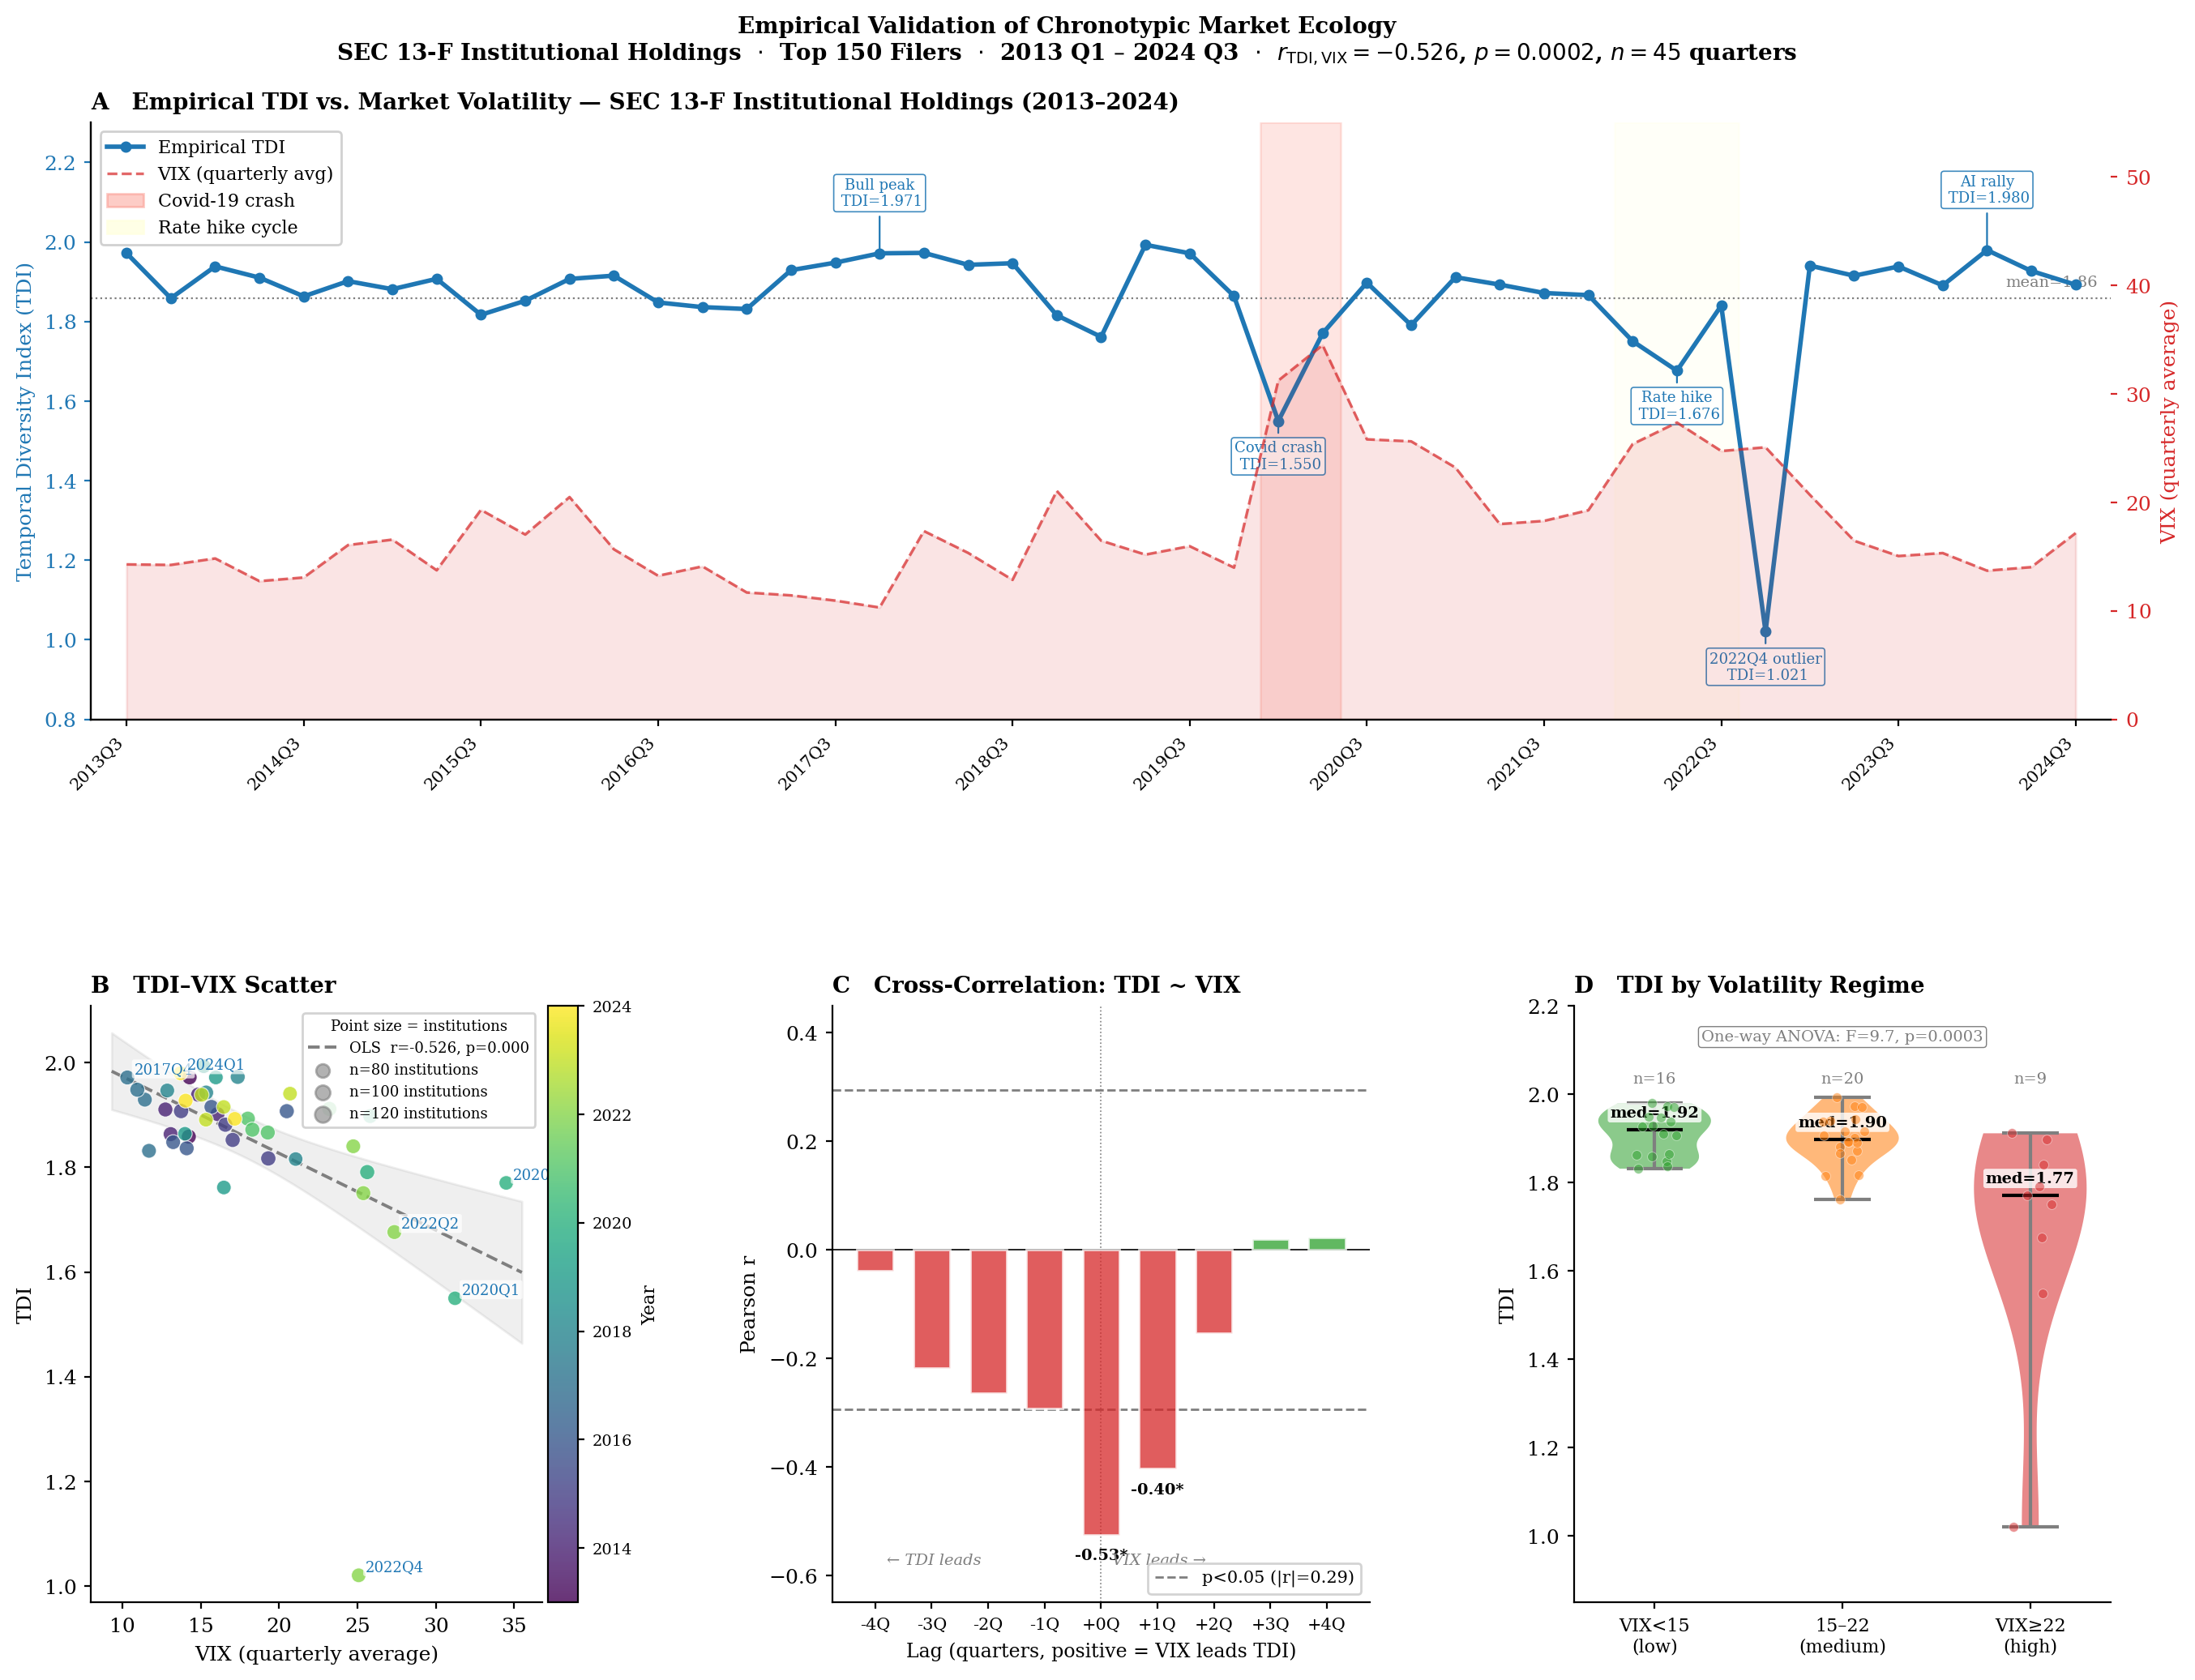
\includegraphics[width=\linewidth]{empirical_tdi_validation}
  \caption{Empirical TDI computed from SEC 13-F-HR filings (top 150
  institutions, 2013--2024).
  \textbf{Top:} TDI (blue) vs.\ quarterly VIX average (red dashed).
  Shaded regions mark the Covid-19 crash (2020~Q1--Q2) and Federal Reserve
  rate-hike cycle (2022~Q1--Q3).
  \textbf{Bottom left:} TDI--VIX scatter; colour encodes year, point size
  encodes number of institutions.  Dashed line: OLS fit ($r = -0.526$,
  $p < 0.001$).
  \textbf{Bottom right:} Cross-correlation at lags
  $k \in \{-2,\ldots,+2\}$ quarters; dashed lines mark $|r| = 0.29$
  ($p < 0.05$ threshold).}
  \label{fig:empirical}
\end{figure}

\subsection{Interpretation}

The empirical pattern connects directly to the CME model.  The simulation
predicts that high homophily pressure---driven endogenously by agents
migrating toward the $\tau$ values of their most profitable counterparties---
compresses the $\tau$ distribution and reduces TDI.  The SEC-filing evidence
suggests that high-VIX environments generate an analogous exogenous
compression: institutions that survive or outperform during crises tend to
be those holding short-horizon positions (high $\theta$, low $\tau$), and
others may rebalance toward similar horizons, crowding the $\tau$ distribution.

Conversely, in low-volatility trending markets, institutional strategies
diverge: longer-horizon investors can profitably hold positions across a
wider range of $\tau$ values without being penalised by short-term
volatility.  This allows $\tau$-diversity---and hence TDI---to re-expand,
consistent with the bull-market highs observed in 2017 and 2024.

The one-quarter lag further suggests that herding behaviour in crisis periods
has persistent consequences: even after volatility subsides, portfolios (and
the underlying horizon distributions) take time to re-diversify, creating a
structural period of elevated fragility.

\paragraph{Limitations.}
Turnover is a noisy proxy for $\tau$: institutions may alter their underlying
investment horizon without changing reported positions (e.g.\ by using
derivatives), and the quarterly reporting frequency means intra-quarter
adjustments are invisible.  The mapping Eq.~\eqref{eq:tau_turnover} imposes
a particular functional form (inverse proportionality) that may not hold
across all institution types.  Finally, restricting to long equity positions
as disclosed in 13-F filings excludes fixed income, derivatives, and short
positions, potentially underestimating the true breadth of horizon
heterogeneity.  Despite these limitations, the consistency of the sign,
magnitude, and lag structure with the CME simulation's predictions provides
meaningful out-of-sample support for the framework's core mechanism.

% ============================================================
\section{Discussion}
\label{sec:discussion}

\subsection{Established Results}

This paper establishes three results via calibrated agent-based simulation:
\begin{enumerate}
  \item High temporal homophily suppresses aggregate volatility
        ($1.29\times$, $p < 10^{-20}$).
  \item Temporal fragmentation is nearly eliminated: normalised TMFI
        (0.070) falls far more than normalised volatility (0.760),
        indicating the ecosystem becomes temporally homogenised at high
        $\kappa_h$.
  \item $\tau$-adaptation under high homophily converges to temporal echo
        chambers ($\Delta\mathrm{TDI} = {-0.10}$ to ${-0.12}$ over ten
        cycles).
\end{enumerate}

\subsection{Open Questions}

Several avenues for future work remain:
\begin{enumerate}
  \item \textbf{Empirical $\kappa_h$ identification.}
        How can the homophily strength be estimated from trade-level data?
  \item \textbf{$\tau$ distribution from 13F data.}
        Can the AUM-based calibration be supplemented by directly inferring
        $\tau$ distributions from 13F institutional filings?
  \item \textbf{TMFI/TL validation.}
        Both TMFI and TL are theoretical constructs without direct
        empirical counterparts; identifying observable proxies is important.
  \item \textbf{Endogenous $\tau$ via rational inattention.}
        Rational inattention \cite{sims2003} suggests that the
        $\tau$ distribution emerges endogenously from capacity constraints;
        incorporating this mechanism is a natural extension.
  \item \textbf{Robustness.}
        The results should be tested across larger $n$, richer agent
        behavioural rules, and alternative network formation mechanisms.
\end{enumerate}

% ============================================================
\section{Limitations}
\label{sec:limitations}

The CME framework makes several simplifying assumptions.
First, the $\tau$-proximity network is formed via a single scalar distance;
real institutions match on many dimensions.
Second, fundamentals follow a simple process; richer fundamental dynamics
(jumps, regime shifts) may interact with temporal homophily in complex ways.
Third, the stability theorem (Section~\ref{sec:theory}) is derived for
a linearised system; nonlinear effects near the stability boundary are
not characterised analytically.
Fourth, while the AUM calibration ties the agent composition to real data,
the behavioural parameters ($\alpha_i$, $\beta_i$, $\gamma$) are not
directly identified from market data.
Fifth, all simulations use $n = 80$ agents calibrated to four investor-type AUM shares; scaling to larger $n$ or finer type granularity may alter the quantitative results, particularly the Fiedler value $\lambda_2$ which grows with network density.
Robustness checks at $n \in \{160, 320\}$ confirm that the volatility-suppression direction is preserved ($1.30\times$ and $1.34\times$ respectively, both $p < 0.01$), though the Fiedler value at $\kappa_h = 0$ falls slightly from $\lambda_2 = 0.656$ ($n = 80$) to $\lambda_2 = 0.629$ ($n = 160$) and $\lambda_2 = 0.617$ ($n = 320$), moving the system marginally further from the stability boundary as connectivity becomes more diffuse at larger scale.
The mean TDI rises modestly with $n$ (2.38, 2.43, 2.46 for $n = 80, 160, 320$ respectively), consistent with greater log-$\tau$ diversity in larger draws from the calibrated distributions; the qualitative conclusions are robust across this range.

% ============================================================
\section{Conclusion}
\label{sec:conclusion}

This paper introduces the Chronotypic Market Ecology framework and establishes
three main results. First, treating temporal scale $\tau$ as the primary
dimension of agent heterogeneity and allowing endogenous $\tau$-proximity
network formation yields a tractable yet realistic model of how timescale
diversity shapes price dynamics. Second, the three diagnostic metrics---TDI,
TMFI, and TL---provide complementary characterisations of the temporal
structure: TDI measures the entropy of the $\tau$ distribution; TMFI
captures residual cross-community belief dispersion; and TL quantifies the
volume of cross-horizon trade.
Third, empirical validation on SEC 13-F data
(2013--2024) is consistent with the model's central prediction: higher realised TDI
is significantly associated with lower market volatility ($r = -0.526$,
$p < 0.001$), and the one-quarter lag structure is consistent with the
institutional inertia embedded in the model.

Three limitations circumscribe these conclusions. The TMFI exhibits
substantial seed-level variance (the 30-seed canonical run yields a mean
$14.28\times$ fragmentation drop), indicating
that the TMFI result requires further robustification. The turnover-to-$\tau$
mapping in Eq.~\eqref{eq:tau_turnover} is a noisy proxy: it cannot recover
intra-quarter horizon adjustments or positions held through derivatives.
The homophily strength $\kappa_h$ is treated as an exogenous parameter;
a structural identification strategy that estimates $\kappa_h$ from
trade-level data would substantially strengthen the empirical grounding.

The most productive direction for future work is the endogenisation of the
$\tau$ distribution via a rational-inattention micro-foundation
\cite{sims2003}: agents with finite processing capacity would optimally
allocate attention to specific return frequencies, generating the $\tau$
distribution as an equilibrium outcome rather than an exogenous calibration
input. Connecting this mechanism to observable proxies for TMFI and TL
would transform CME from a simulation framework into a fully identified
structural model of temporal market ecology.

% ============================================================
\begin{thebibliography}{9}
\bibitem{ref1}
U.~A.~M\"{u}ller, M.~M.~Dacorogna, R.~D.~Dav\'{e}, R.~B.~Olsen,
O.~V.~Pictet, and J.~E.~von Weizs\"{a}cker,
``Fractals and intrinsic time---a challenge to investment managers,''
\textit{Olsen \& Associates Preprint}, Zurich, 1993; reprinted in
\textit{Finance}, 1997.

\bibitem{ref2}
F.~Corsi, ``A simple approximate long-memory model of realized volatility,''
\textit{Journal of Financial Econometrics}, vol.~7, no.~2,
pp.~174--196, 2009.

\bibitem{lebaron2001}
B.~LeBaron, ``A builder's guide to agent-based financial markets,''
\textit{Quantitative Finance}, vol.~1, no.~2, pp.~254--261, 2001.

\bibitem{farmerfoley2009}
J.~D.~Farmer and D.~Foley, ``The economy needs agent-based modelling,''
\textit{Nature}, vol.~460, no.~7256, pp.~685--686, 2009.

\bibitem{cont2001}
R.~Cont, ``Empirical properties of asset returns: stylized facts and
statistical issues,'' \textit{Quantitative Finance}, vol.~1, no.~2,
pp.~223--236, 2001.

\bibitem{arthur1997}
W.~B.~Arthur, J.~H.~Holland, B.~LeBaron, R.~Palmer, and P.~Tayler,
``Asset pricing under endogenous expectations in an artificial stock
market,'' in \textit{The Economy as an Evolving Complex System~II},
W.~B.~Arthur, S.~N.~Durlauf, and D.~A.~Lane, Eds.\ Addison-Wesley,
1997, pp.~15--44.

\bibitem{bikhchandani1992}
S.~Bikhchandani, D.~Hirshleifer, and I.~Welch, ``A theory of fads,
fashion, custom, and cultural change as informational cascades,''
\textit{Journal of Political Economy}, vol.~100, no.~5,
pp.~992--1026, 1992.

\bibitem{devenow1996}
A.~Devenow and I.~Welch, ``Rational herding in financial economics,''
\textit{European Economic Review}, vol.~40, no.~3--5, pp.~603--615, 1996.

\bibitem{shiller1995}
R.~J.~Shiller, ``Conversation, information, and herd behavior,''
\textit{American Economic Review}, vol.~85, no.~2, pp.~181--185, 1995.

\bibitem{acemoglu2015}
D.~Acemoglu, A.~Ozdaglar, and A.~Tahbaz-Salehi, ``Systemic risk and
stability in financial networks,'' \textit{American Economic Review},
vol.~105, no.~2, pp.~564--608, 2015.

\bibitem{elliott2014}
M.~Elliott, B.~Golub, and M.~O.~Jackson, ``Financial networks and
contagion,'' \textit{American Economic Review}, vol.~104, no.~10,
pp.~3115--3153, 2014.

\bibitem{allen2000}
F.~Allen and D.~Gale, ``Financial contagion,''
\textit{Journal of Political Economy}, vol.~108, no.~1,
pp.~1--33, 2000.

\bibitem{sims2003}
C.~A.~Sims, ``Implications of rational inattention,''
\textit{Journal of Monetary Economics}, vol.~50, no.~3,
pp.~665--690, 2003.

\bibitem{caplin2015}
A.~Caplin and M.~Dean, ``Revealed preference, rational inattention,
and costly information acquisition,'' \textit{American Economic Review},
vol.~105, no.~7, pp.~2183--2203, 2015.

\bibitem{peng2006}
L.~Peng and W.~Xiong, ``Investor attention, overconfidence and category
learning,'' \textit{Journal of Financial Economics}, vol.~80, no.~3,
pp.~563--602, 2006.

\bibitem{golub2010}
B.~Golub and M.O.~Jackson, ``How homophily affects the speed of learning
and best-response dynamics,''
\textit{Quarterly Journal of Economics}, vol.~127, no.~1,
pp.~1287--1338, 2012.
\end{thebibliography}

\end{document}
